\documentclass[a4paper, 12pt, finnish]{article}
\usepackage{babel}
\usepackage[utf8]{inputenc}
\usepackage[T1]{fontenc}
\usepackage{graphicx}
\title{Keskustelufoorumin Dokumentaatio}
\author{Timo Mäki}
\date{\today}

\begin{document}
 \maketitle

Tämä on dokumentaatio tietokantasovelluksen harjoitustyön keskustelufoorumiin.

\newpage\null\thispagestyle{empty}\newpage
\tableofcontents
\newpage\null\thispagestyle{empty}\newpage
\section{Johdanto}

Aiheena on luoda keskustelufoorumi.
Foorumissa käyttäjät voivat kirjoittaa viestejä ja lukea muiden kirjoittamia viestejä.
Viestit liittyvät viestiketjuihin, joilla on otsikoita.
Käyttäjät voivat luoda viestiketjuja.
Viestejä tulee voida myös etsiä otsikon, iän tai kirjoittajan perusteella. Käyttäjillä on yksityiset tunnukset, joilla he voivat kirjautua sisään.
Tunnukset tarvitaan, jotta voi kirjoittaa viestin foorumille.
Jokaisella käyttäjätunnuksella voi kirjoittaa viestejä.
Pääkäyttäjällä on oikeus viedä käyttäjän oikeus kirjoittaa viestejä, sekä poistaa viestejä, että viestiketjuja.
\indent

Foorumin tarkoitus on edistää sosiaalista kanssakäyntiä ihmisten välillä, auttaa samanhenkisiä ihmisiä löytämään toisensa ja antaa ihmisten sekä anonyymisti että toisia kunnioittavasti esittää mielipiteitään internetin välityksellä.
\indent

Järjestelmän tavoitteet ovat mahdollistaa viestien kirjoitus ja luku, käyttäjätunnusten luonti, käyttöoikeus ryhmien olemassaolo sekä mahdollistaa nopea viestin haku.
\indent

Järjestelmä pyörii tktl:n users palvelimella, apachea käyttäen.
Se vaatii PHP-tuen.
Käyttäjän selaimelta edellytetään todennäköisesti javascript tukea.
Järjestelmä edellyttää PostgreSQL tietokantaa.
On todennäköistä, että, rajapintoja hyödyntäen, tietokanta tulee olemaan silti helppo vaihtaa.

\newpage
\section{Yleiskuva järjestelmästä}
\subsection{Jokamies}
Jokamies on henkilö, joka ei ole välttämättä rekisteröitynyt tai kirjautunut sisään.
Jokainen foorumin käyttäjä on jokamies.

\begin{itemize}
\item
Voi lukea foorumille tehtyjä kirjoituksia.

\item
Voi hakea viestejä.

\item
Voi rekisteröityä.

\item
Voi kirjautua foorumiin.
\end{itemize}

\subsection{Rekisteröitynyt käyttäjä}
Rekisteröitynyt käyttäjä on henkilö, joka on rekisteröinyt tunnuksen foorumille.

\begin{itemize}
\item
    Voi aloittaa uuden viestiketjun.
\item
    Voi vastata olemassa olevaan viestiketjuun.
\item
    Näkee kirjoitukset, joita henkilö ei ole vielä lukenut.
\end{itemize}

\subsection{Pääkäyttäjä}
Pääkäyttäjä on henkilö, joka vastaa foorumin ylläpidosta.
Tämä on erityisryhmä ja on oletusarvoisesti vain foorumin perustajalla. Pääkäyttäjällä on myös rekisteröityneen käyttäjän oikeudet.

\begin{itemize}
\item
Voi poistaa foorumille kirjoitetun viestin tai viestiketjun.
\item
Voi laittaa eston käyttäjälle, jolloin tämä ei voi enää kirjoittaa uusia viestejä foorumille.
\item
Voi antaa pääkäyttäjän oikeudet muille rekisteröityneille käyttäjille.
\end{itemize}


\section{Käyttötapauskaavio}
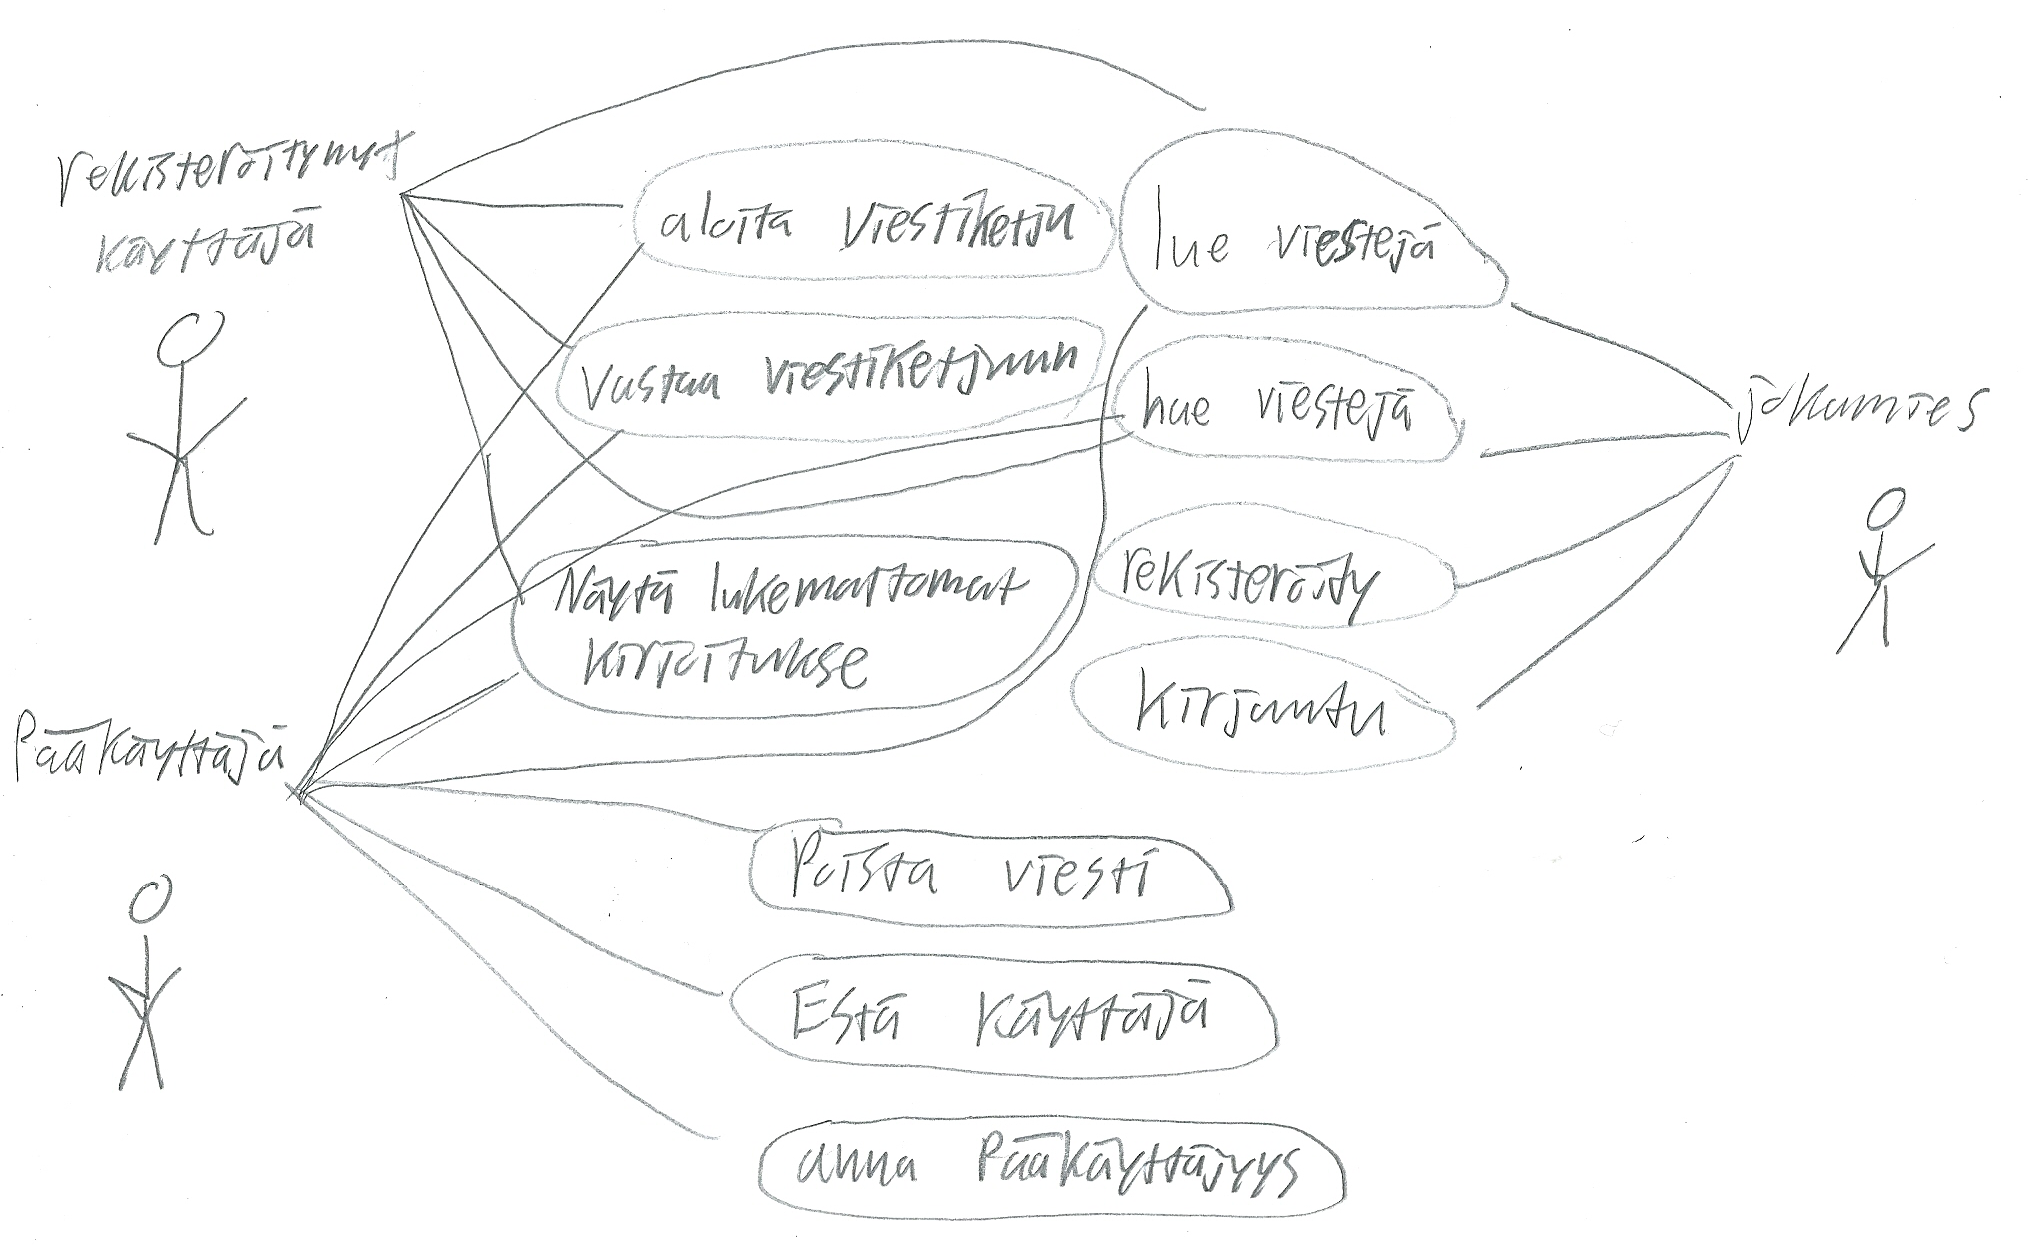
\includegraphics[width=\textwidth,height=\textheight,keepaspectratio]{kayttotapauskaavio.png}

\section{Järjestelmän tietosisältö}
\subsection{Käsitekaavio}
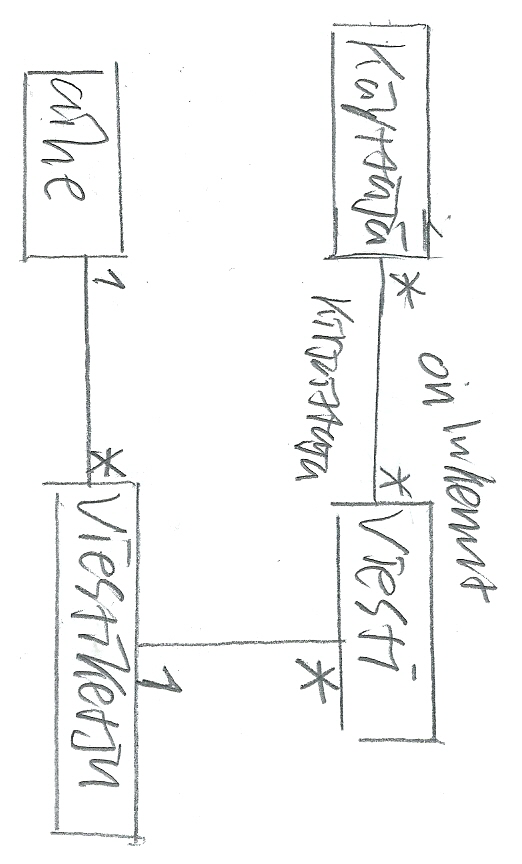
\includegraphics[width=\textwidth,height=\textheight,keepaspectratio]{kasitekaavio.png}

\subsection{Tietosisältö}
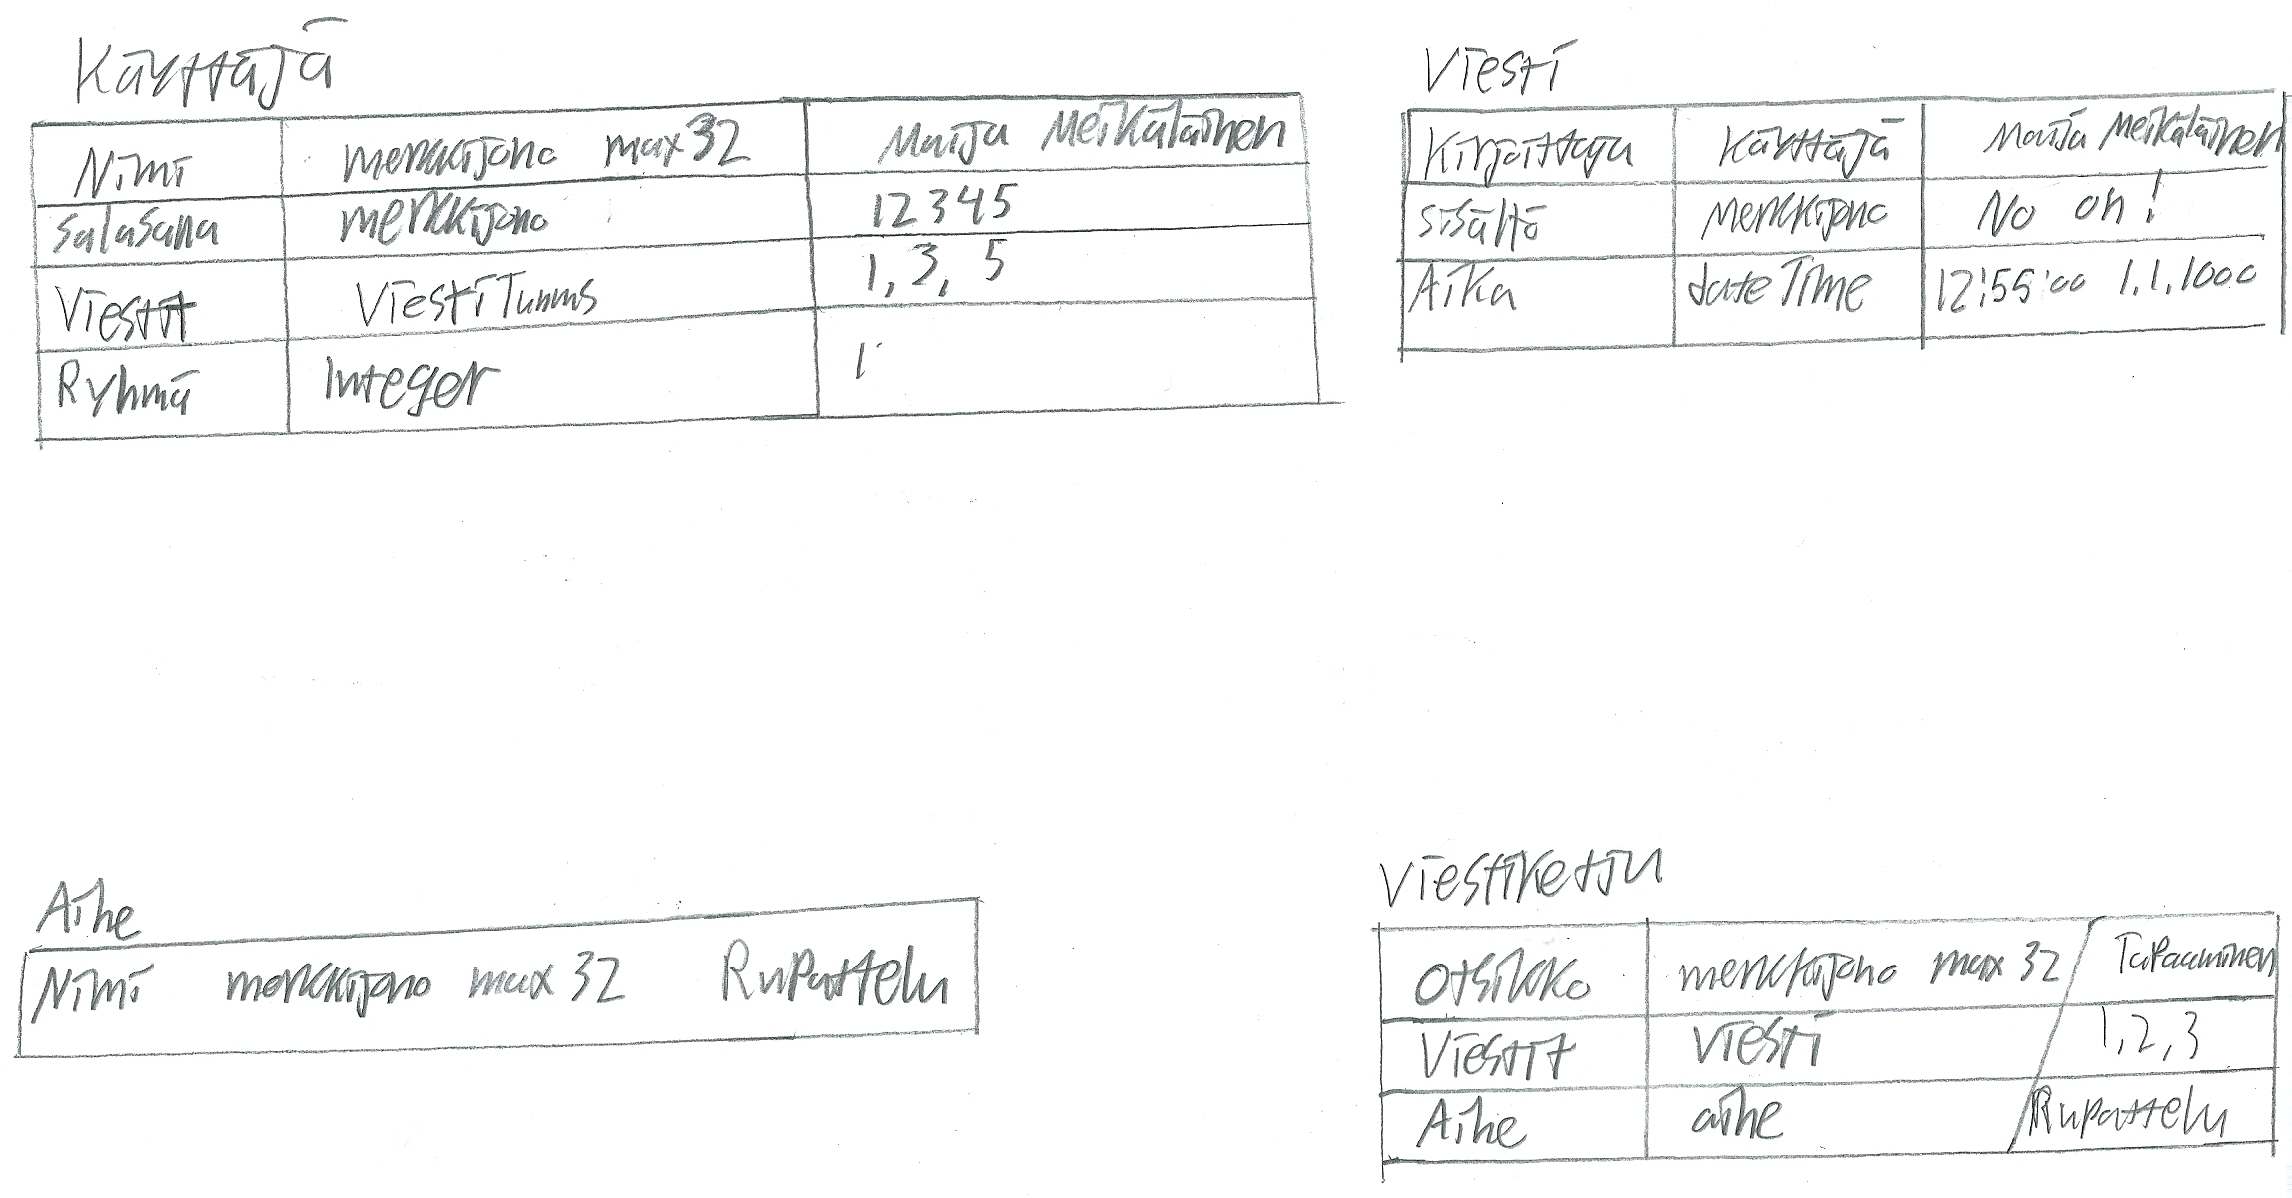
\includegraphics[width=\textwidth,height=\textheight,keepaspectratio]{tietosisalto.png}

\section{Käyttöliittymä}
\subsection{Sivukartta}
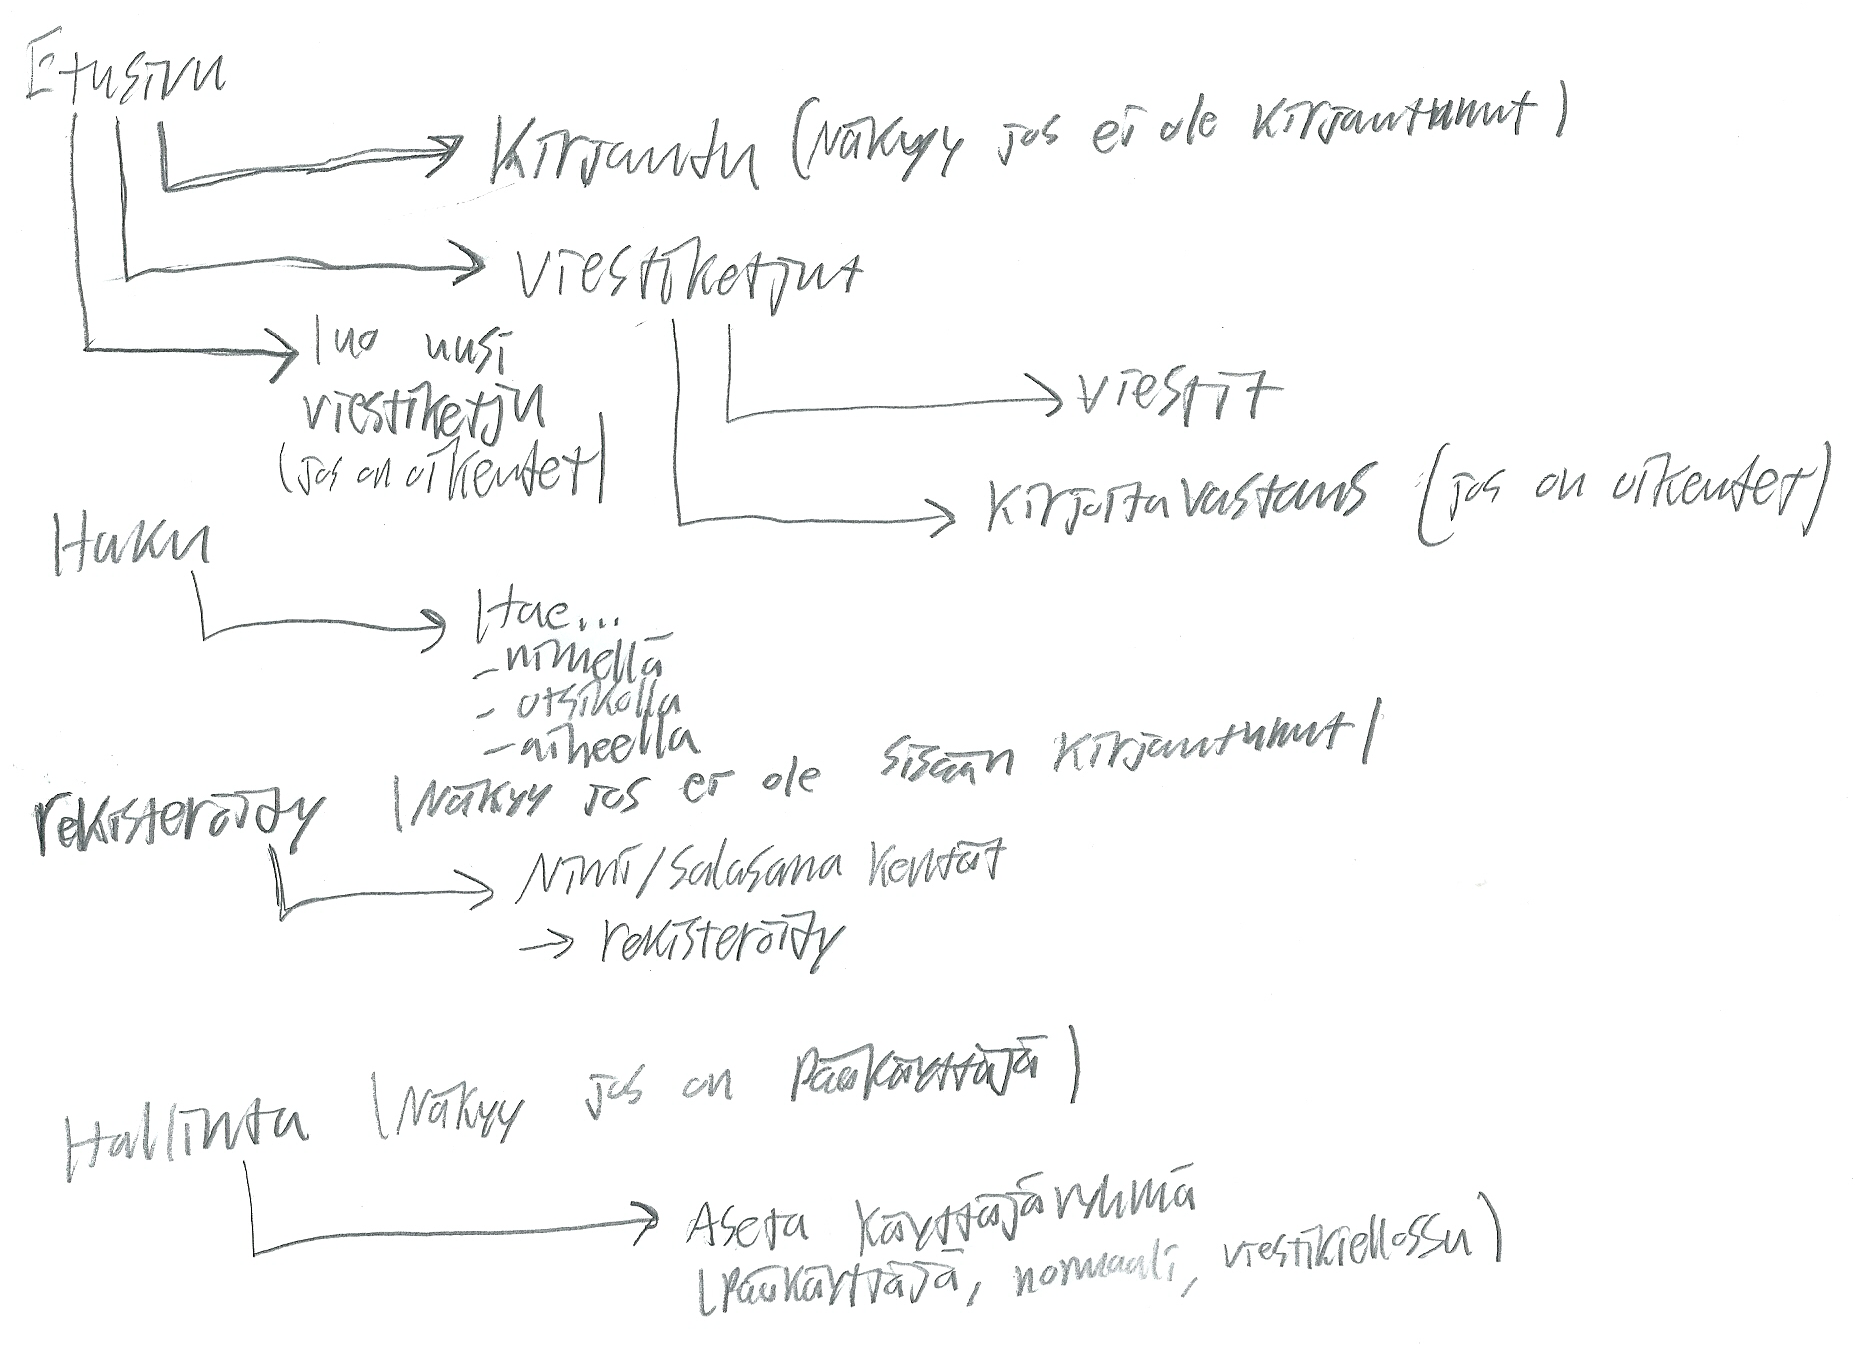
\includegraphics[width=\textwidth,height=\textheight,keepaspectratio]{kayttoliittymakaavio.png}

\subsection{Etusivu}
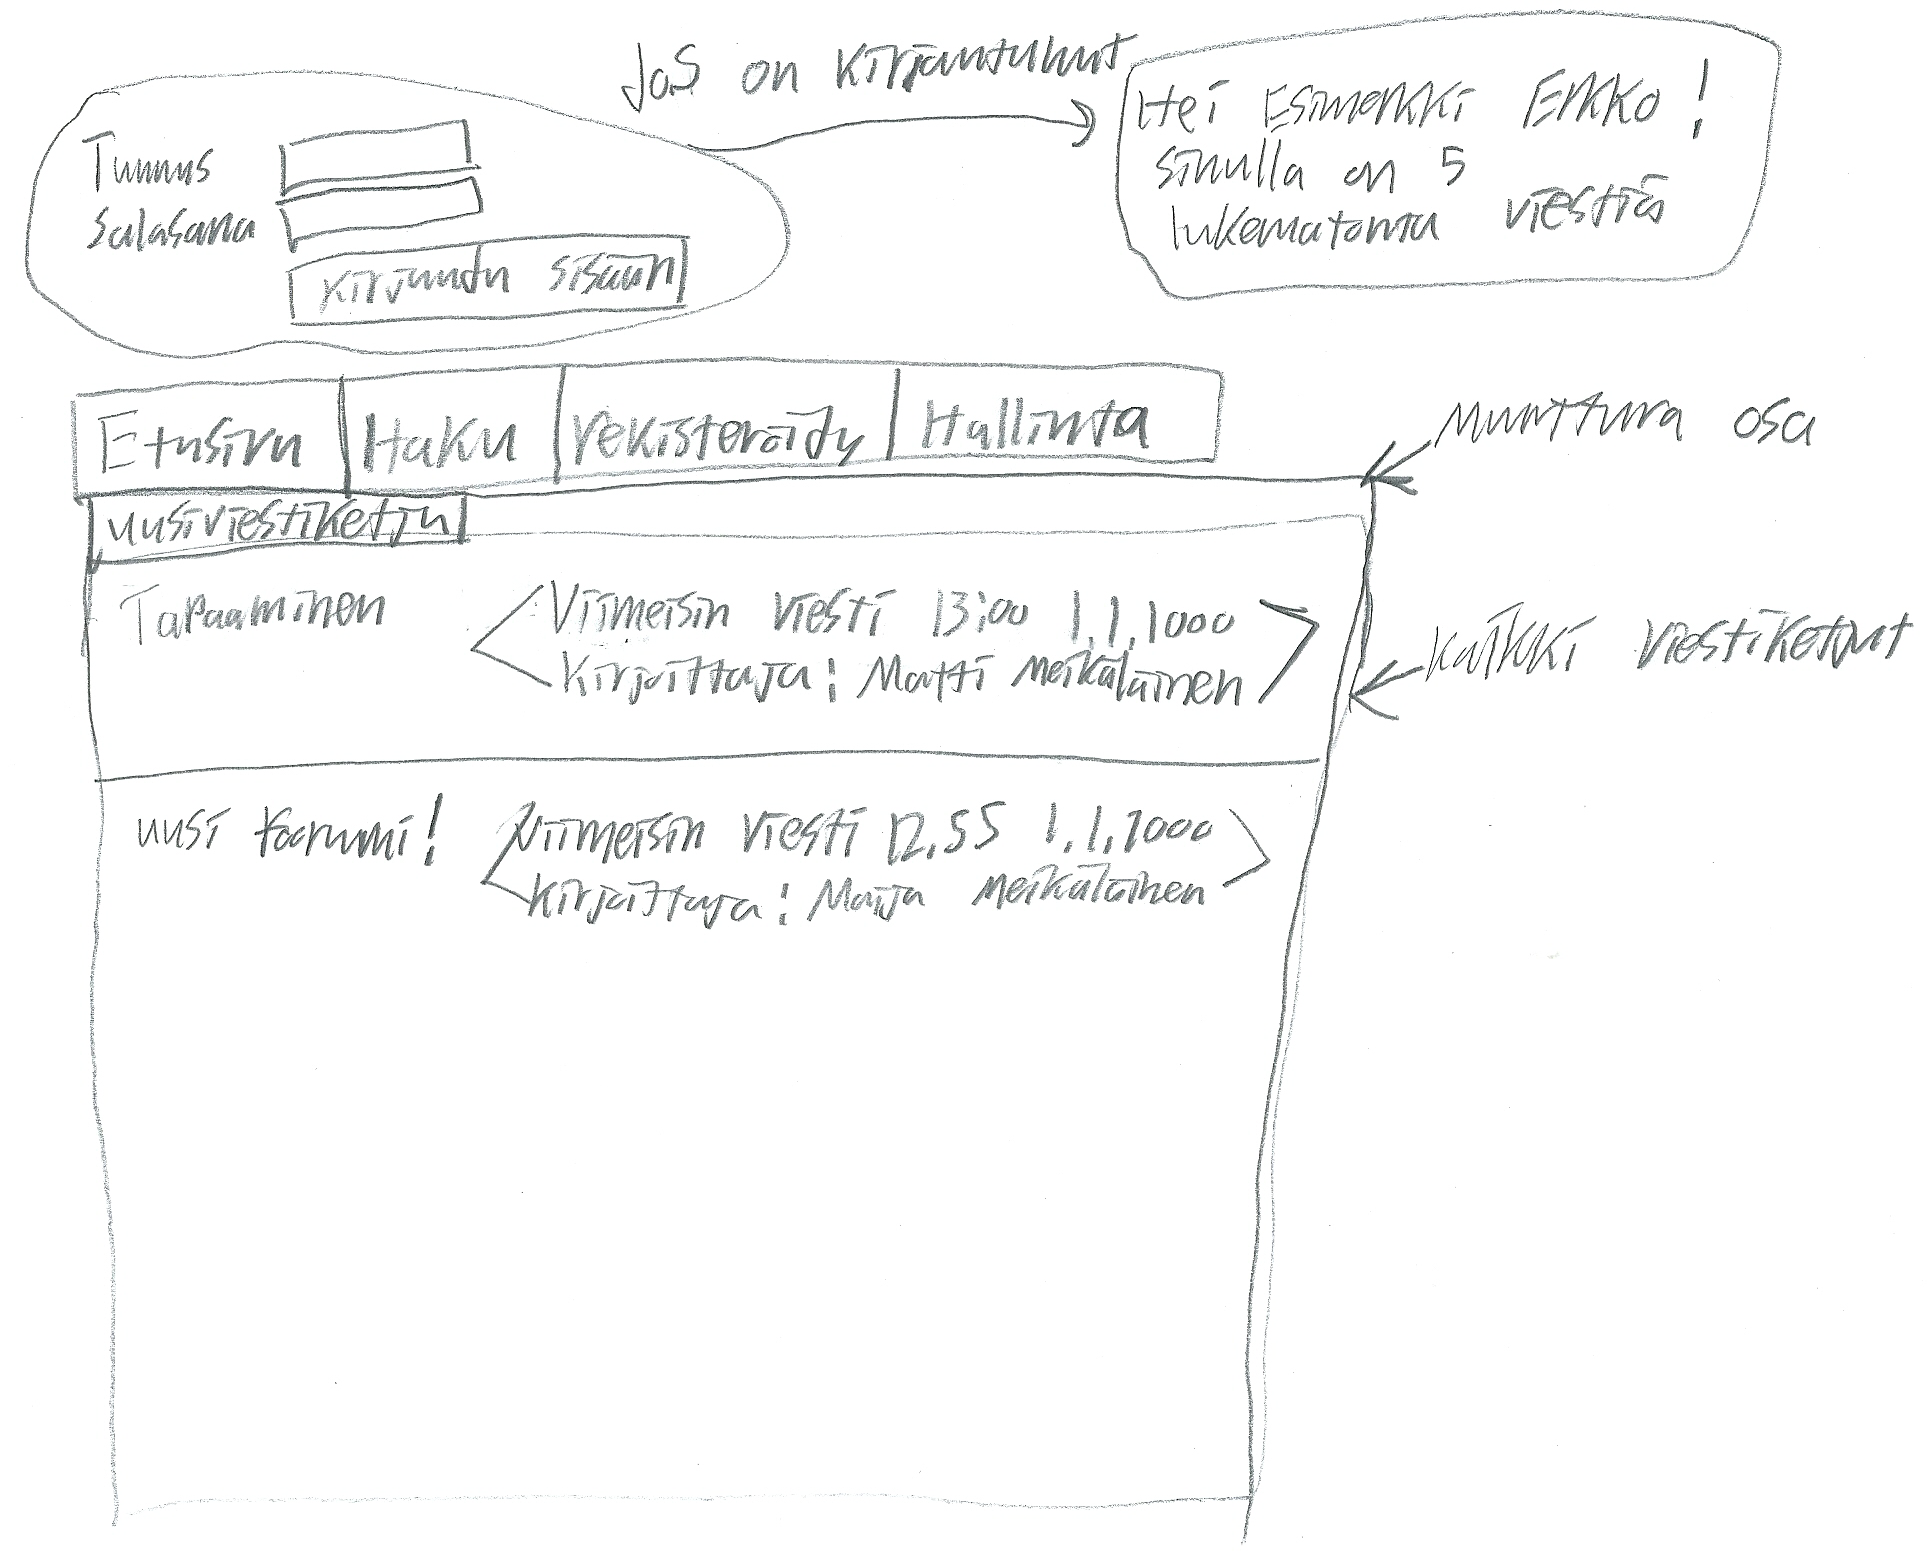
\includegraphics[width=\textwidth,height=\textheight,keepaspectratio]{etusivu.png}

\subsection{Haku}
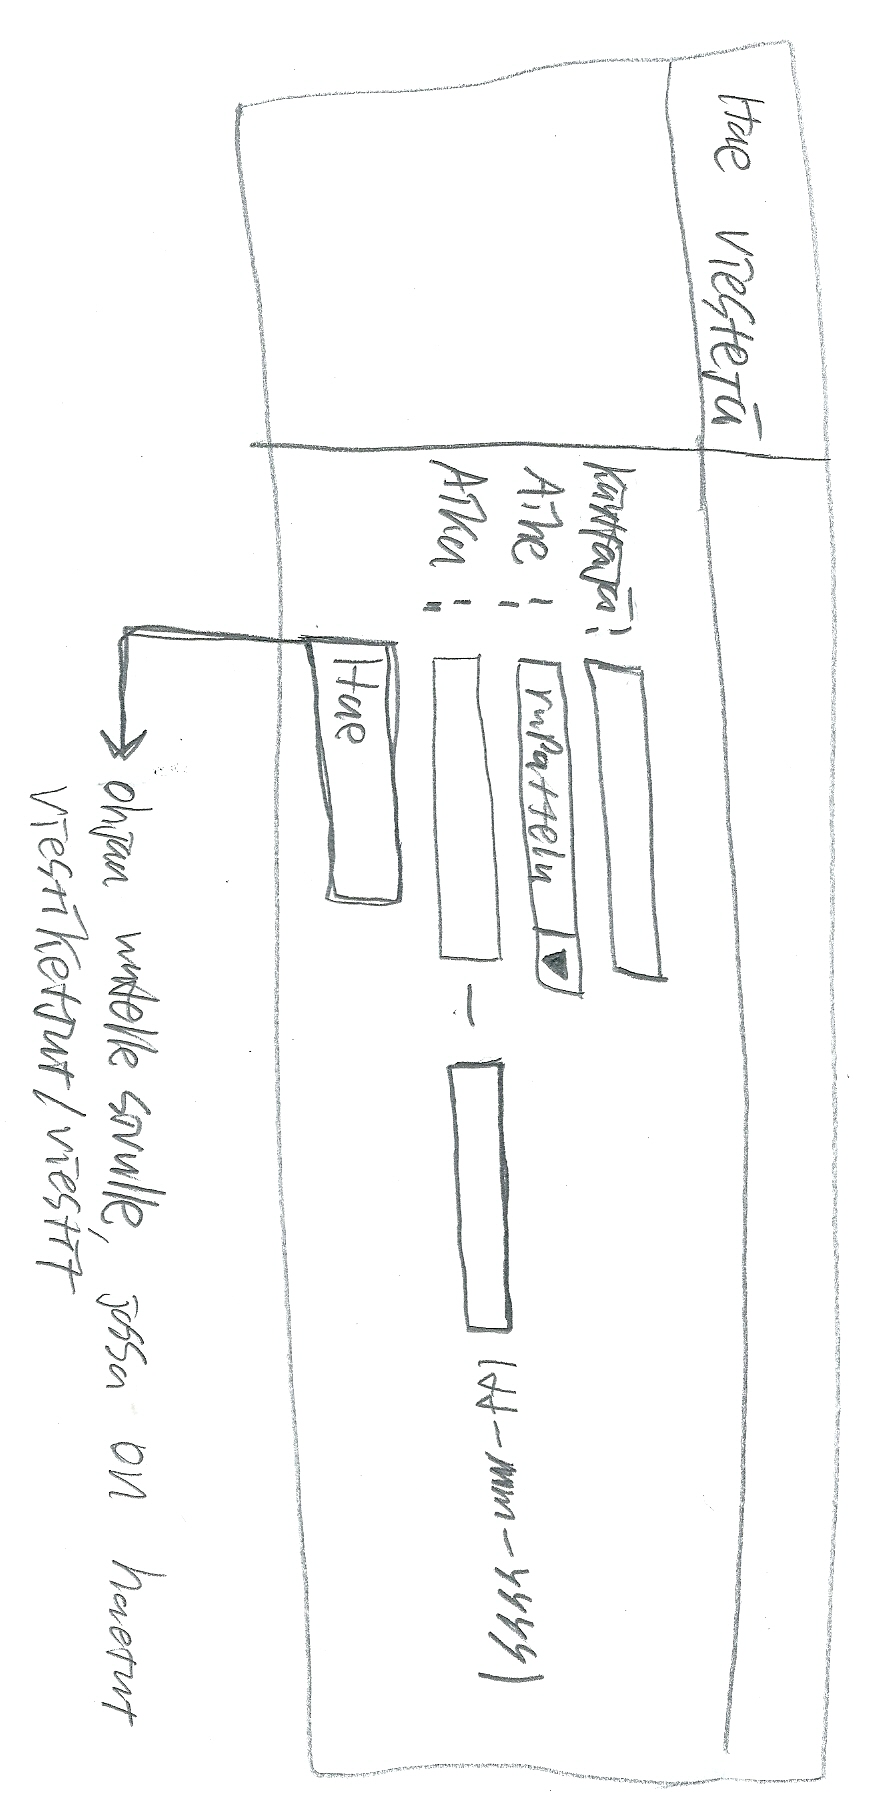
\includegraphics[width=\textwidth,height=\textheight,keepaspectratio]{haku.png}

\subsection{Hallinta}
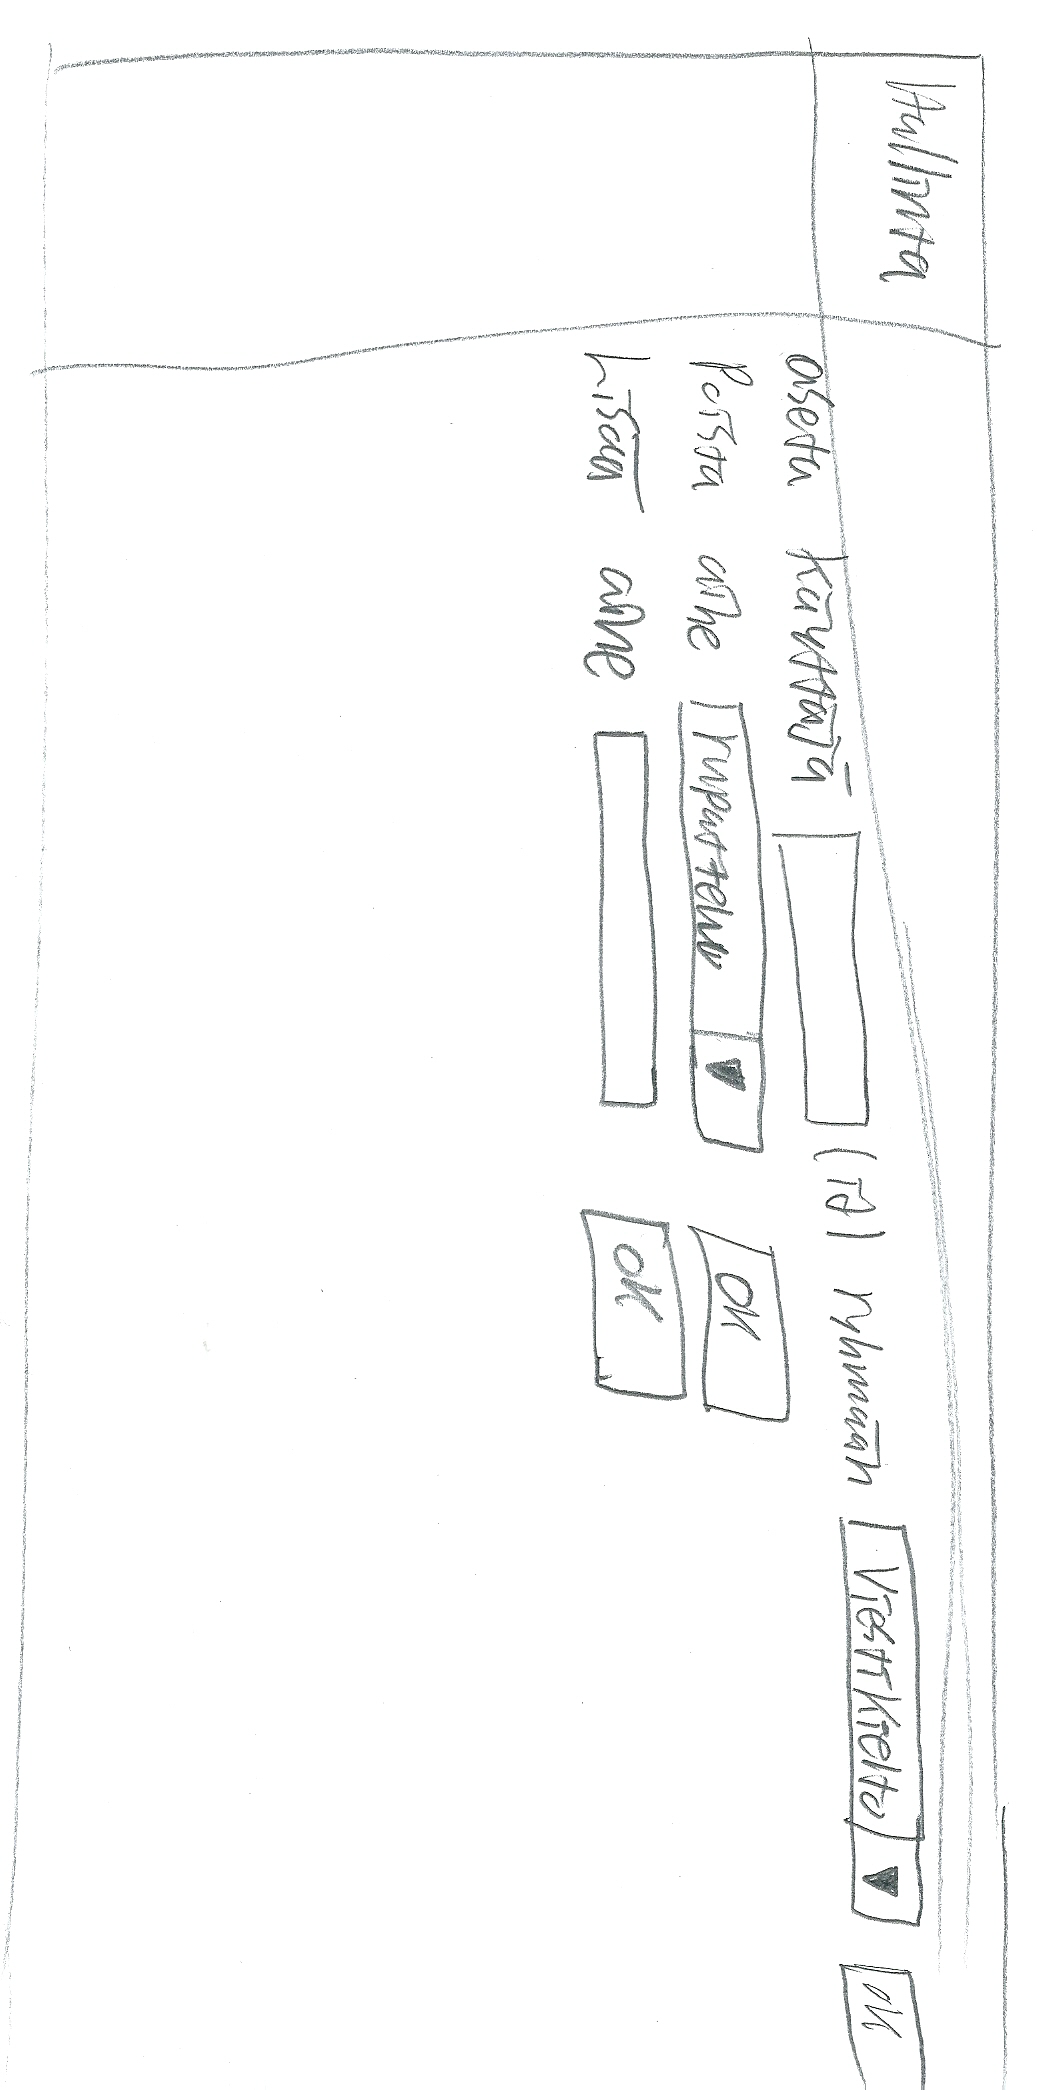
\includegraphics[width=\textwidth,height=\textheight,keepaspectratio]{hallinta.png}

\subsection{Rekisteröityminen}
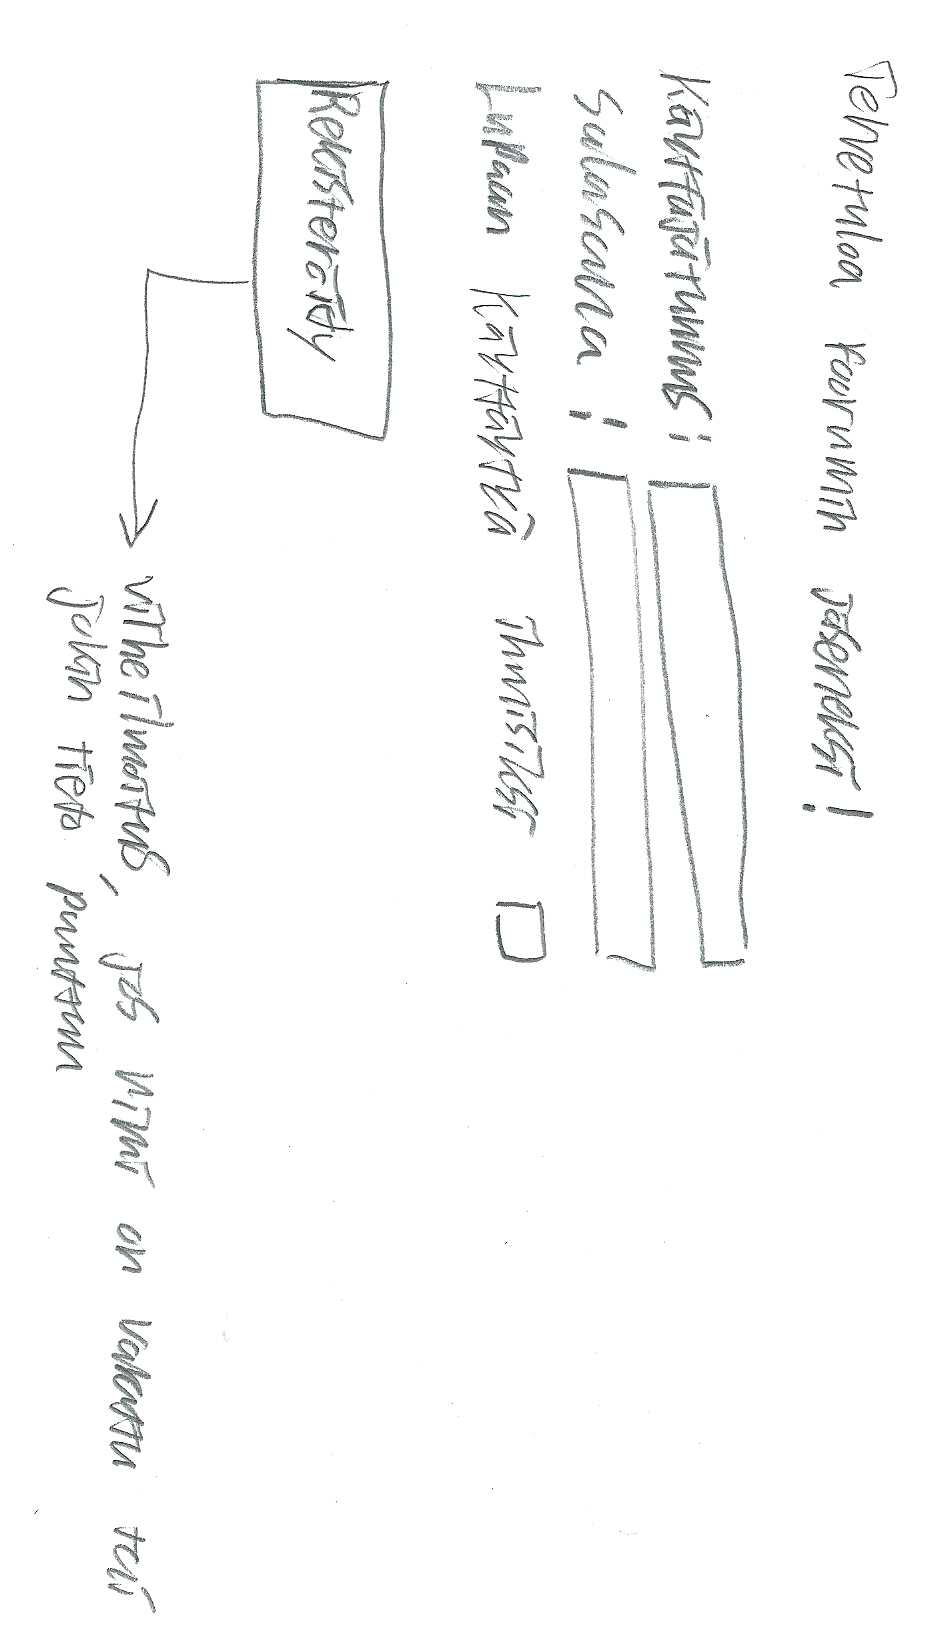
\includegraphics[width=\textwidth,height=\textheight,keepaspectratio]{rekisteroityminen.png}

\subsection{Uusiketju}
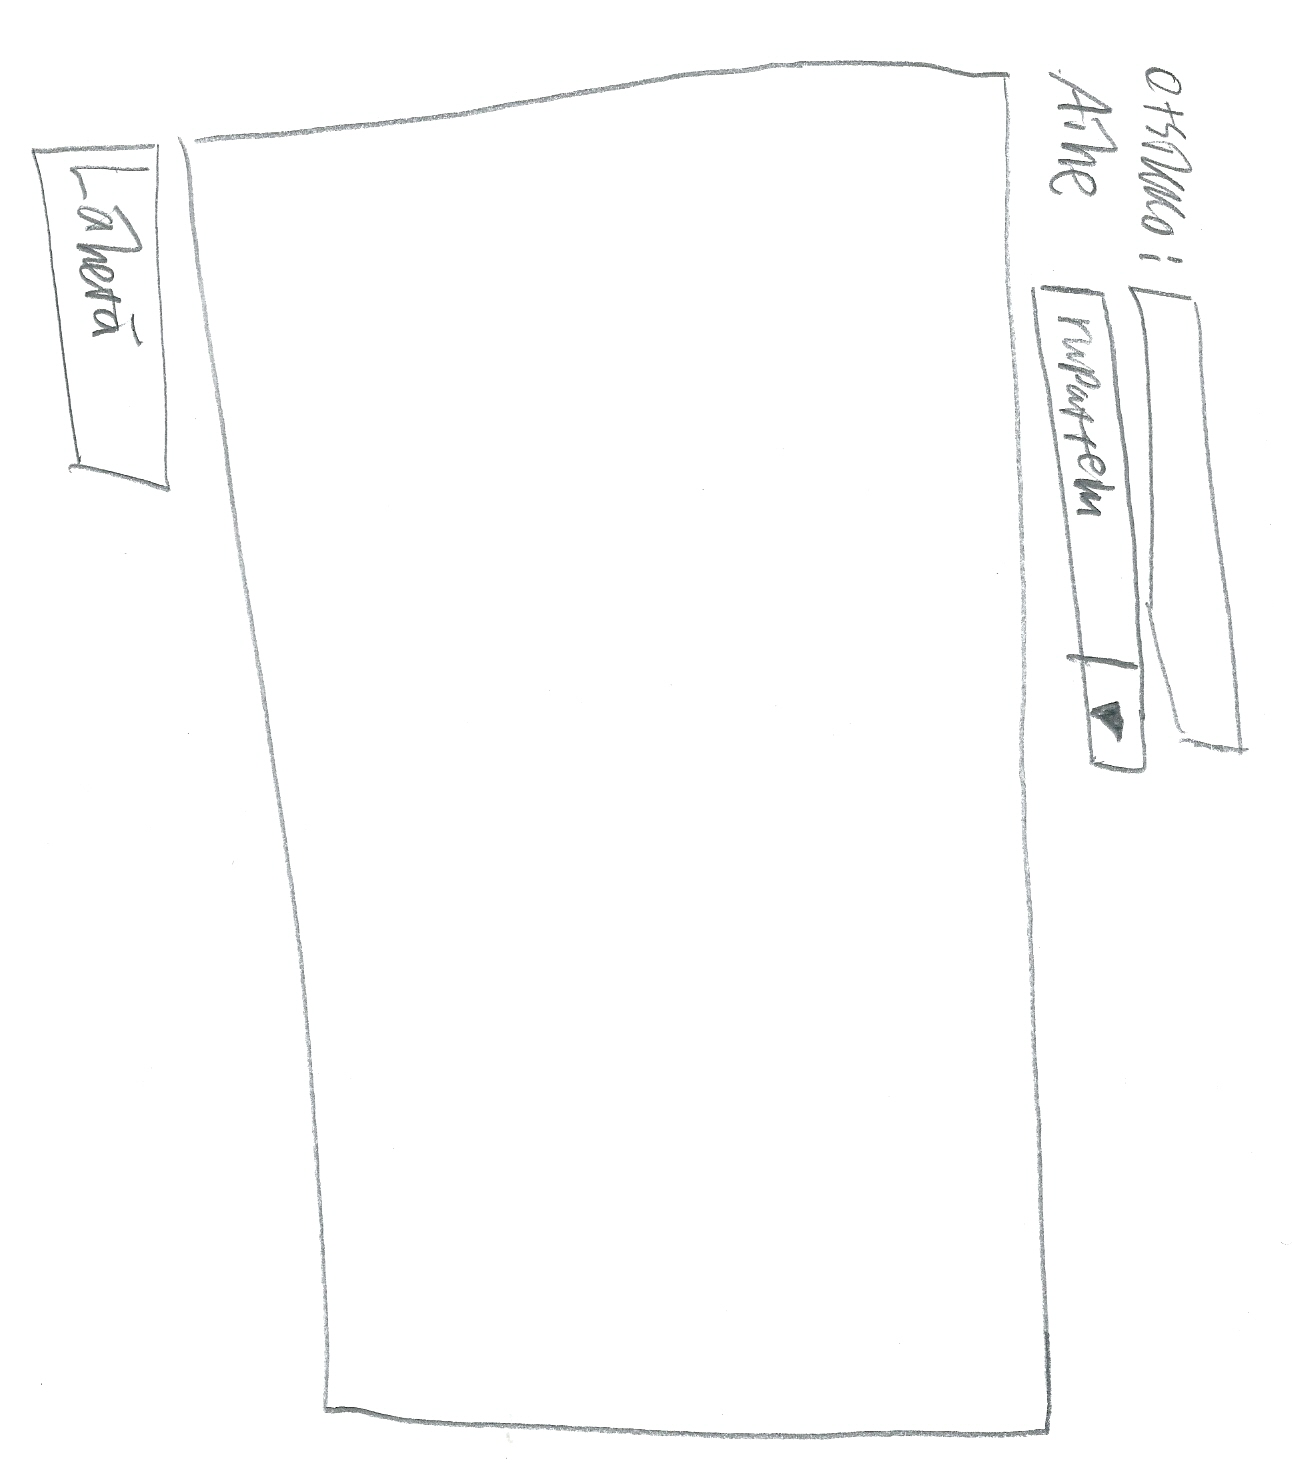
\includegraphics[width=\textwidth,height=\textheight,keepaspectratio]{uusiketju.png}

\subsection{Viestiketju}
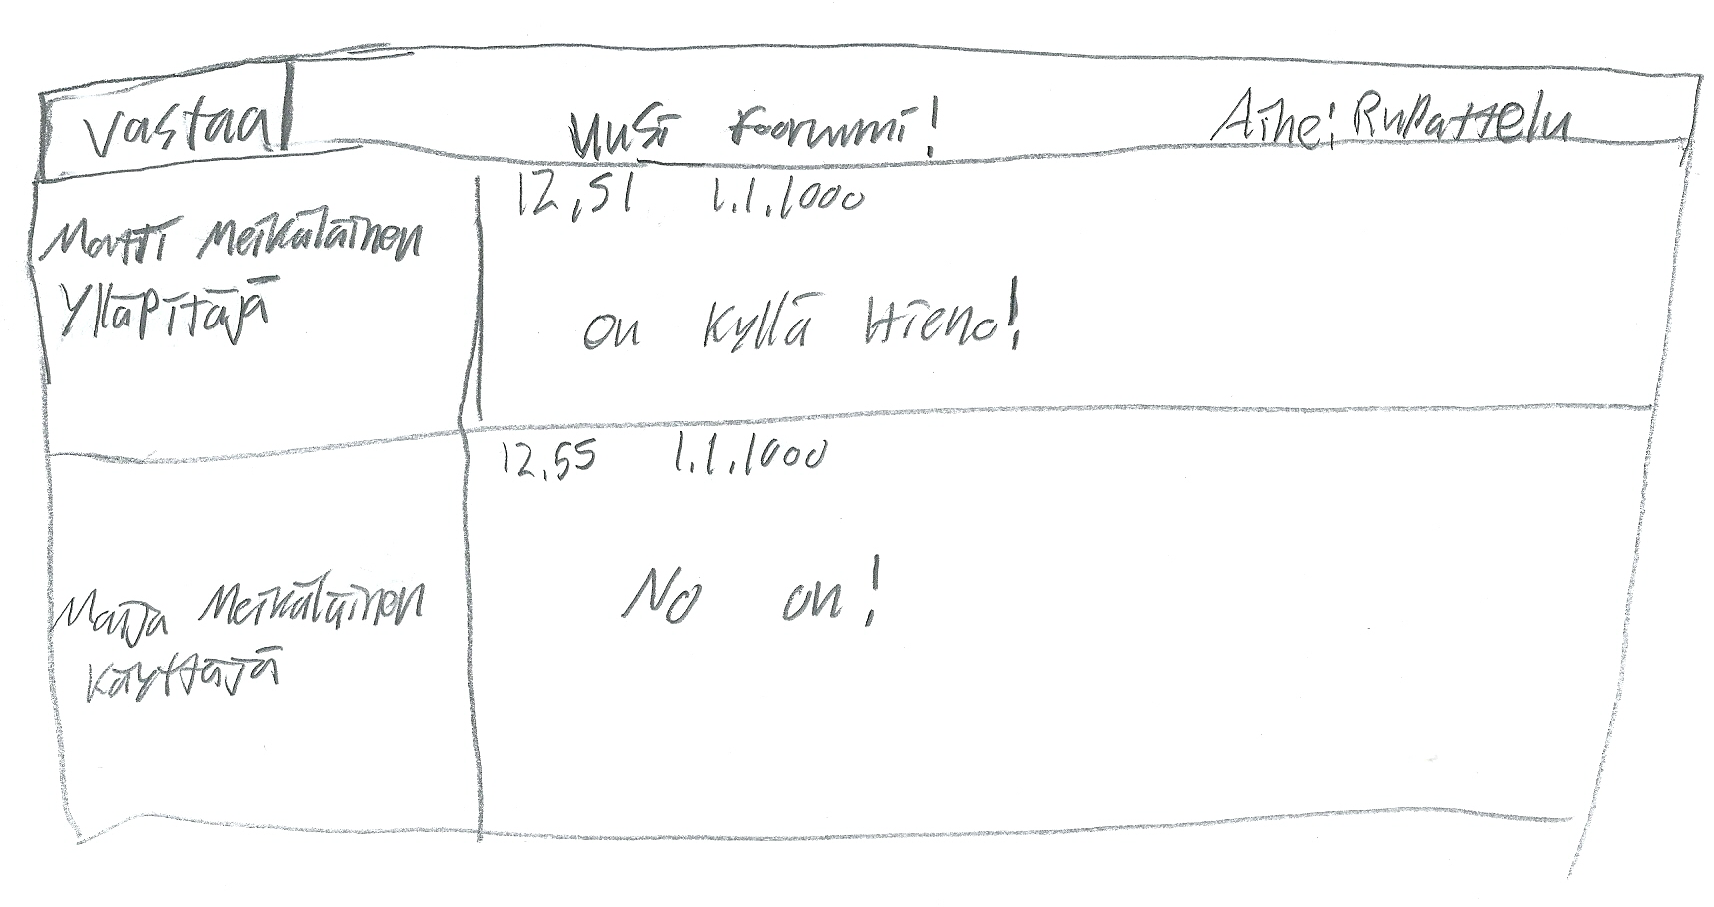
\includegraphics[width=\textwidth,height=\textheight,keepaspectratio]{viestiketju.png}

\subsection{Vastaus}
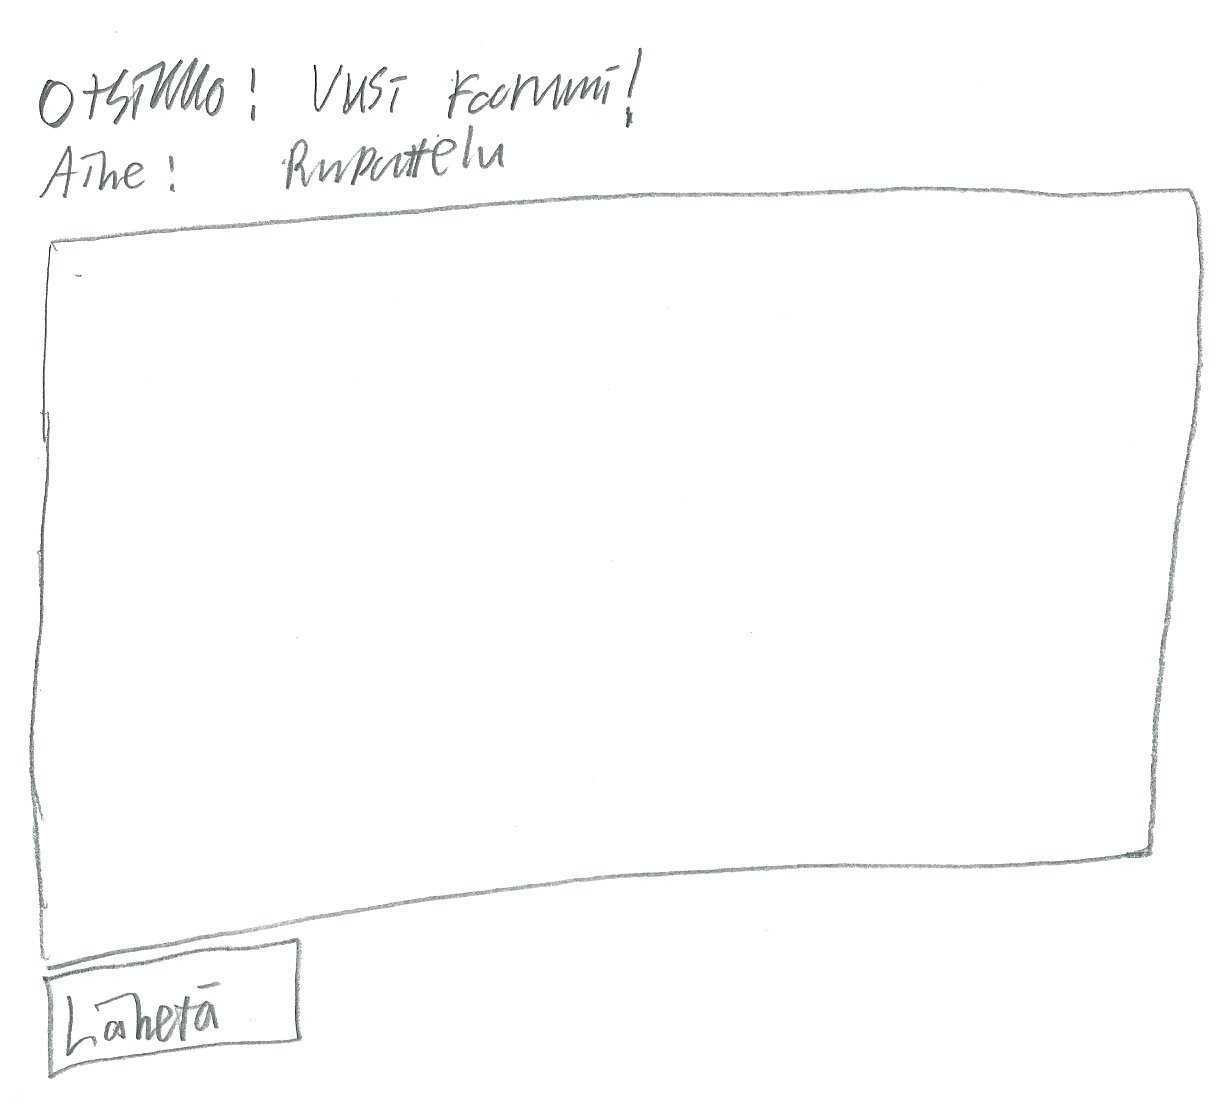
\includegraphics[width=\textwidth,height=\textheight,keepaspectratio]{vastaus.png}

\end{document}
